\section{Mechanizm budowania oraz zarządzanie zasobami w Warhammer 40,000: Dawn of War (Bogna Lew)}

Warhammer 40,000: Dawn of War jest grą typu RTS osadzoną w uniwersum gry bitewnej Warhammer 40,000. Udostępnia
ona tryb jednoosobowy oraz wieloosobowy dla maksymalnie sześciu graczy. W pierwszym wariancie gracz wciela się w postać dowódcy
armii Space Marines z Blood Ravens i ma za zadanie zapobiec inwazji Orków. Gra Warhammer 40,000: Dawn of War bardzo szybko
zyskała na popularności i oferowała wszystko, co było potrzebne dla tego gatunku. Z tego powodu warto się jej przyjrzeć,
pomimo faktu, że jej realia znacząco odbiegających od tych, w których zostanie osadzona tworzona przez nas gra.

Warhammer 40,000: Dawn of War wyróżnia model pozyskiwania surowców. W grze dostępne są dwa rodzaje: Energia, która jest
generowana przez dedykowane do tego budowle oraz Rekwizycja, której szybkość wytwarzania jest uzależniona od kontrolowanych
przez gracza punktów strategicznych. Taka mechanika znacznie lepiej wpasowuje się w realia gry oraz wymusza na użytkowniku
przyjęcie agresywniejszej strategii.

Dodatkowo Warhammer 40,000: Dawn of War posiada typowy dla gier RTS mechanizm tworzenia budowli. Gracz ma
do dyspozycji jednostki, którym może zlecić budowę wybranego przez siebie obiektu po poniesieniu kosztów jego utworzenia.
Zanim będzie możliwe rozpoczęcie budowania użytkownik musi wybrać miejsce, w którym budynek powstanie. Robi to, przesuwając
jego podgląd po mapie. W tym czasie gra dokonuje walidacji miejsca i informuje gracza czy wybrany obszar jest poprawny,
odpowiednio podświetlając widok budynku. Wybudowanie obiektu nie jest natychmiastowe, co sprawia, że gra lepiej oddaje
realia, w których jest osadzona.

\begin{figure}[h!]
    \centering
    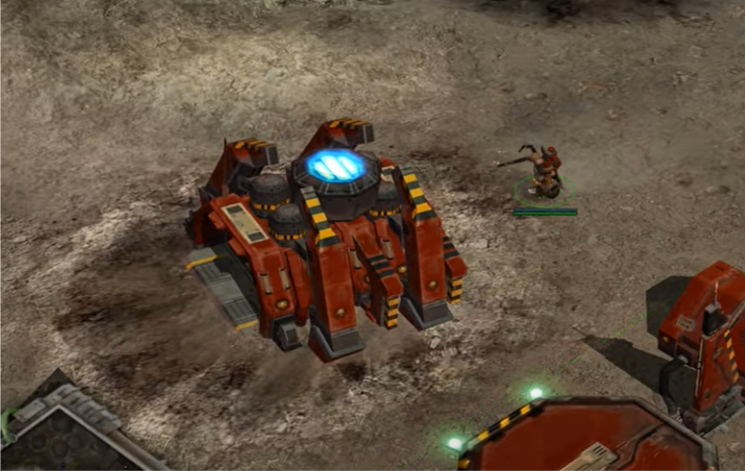
\includegraphics[width=0.9\textwidth]{images/warhammer.png}
    \caption{Budowanie budynku przez dedykowaną do tego jednostkę}
\end{figure}